
\documentclass[12pt]{article}
\usepackage[english,finnish]{babel}
\usepackage{t1enc}

% AMS packages:
\usepackage{amsbsy}
\usepackage{amsfonts}
\usepackage{amsmath}
\usepackage{amssymb}
\usepackage{amsthm}
\usepackage{amsxtra}
% for comments to work
\usepackage{verbatim}
\usepackage{hyperref}
\usepackage{graphicx}

%%%%%%%%%%%%%%%%%%%%%%%%%%%%%%%%%%%

% Hilbert spaces:
\newcommand{\hilb}{\mathcal{H}}
\newcommand{\banH}{\mathcal{B}(\hilb)}
\newcommand{\fock}{\mathcal{F}}

% Products:
\newcommand{\scalpr}[2]{( #1, #2 )}
\newcommand{\dualpr}[2]{\langle #1, #2 \rangle}

% Fonts
\newcommand{\calc}{\mathcal{C}}
\newcommand{\cala}{\mathcal{A}}
\newcommand{\calv}{\mathcal{V}}
\newcommand{\calf}{\mathcal{F}}
\newcommand{\cals}{\mathcal{S}}
\newcommand{\cald}{\mathcal{D}}
\newcommand{\banach}{\mathcal{B}}
\newcommand{\id}[1]{\mathbbm{1}\!\left({#1}\right)}

\newcommand{\ci}{{\rm i}}
\newcommand{\rmd}{{\rm d}}
\newcommand{\rme}{{\rm e}}

\newcommand{\re}{{\rm Re\,}}
\newcommand{\im}{{\rm Im\,}}

% misc
\newcommand{\defem}[1]{{\em #1\/}}
\newcommand{\vep}{\varepsilon}


\newcommand{\qand}{\quad\text{and}\quad}

% To define sets:
\newcommand{\defset}[2]{ \left\{ #1 \left|\, #2\makebox[0pt]{$\displaystyle\phantom{#1}$}\right.\!\right\} }

\newcounter{alplisti}
\renewcommand{\thealplisti}{\alph{alplisti}}
\newenvironment{alplist}[1][(\thealplisti)]{\begin{list}{{\rm #1}\ }{ %
      \usecounter{alplisti} %
    \setlength{\itemsep}{0pt}
    \setlength{\parsep}{0pt}  %
%    \setlength{\leftmargin}{5em} %
%    \setlength{\labelwidth}{5em} %
%    \setlength{\labelsep}{1em} %
%    \settowidth{\labelwidth}{(DR2)}
     \setlength{\topsep}{0pt} %
}}{\end{list}}

% Norms:
\newcommand{\abs}[1] {\lvert #1 \rvert}
\newcommand{\norm}[1]{\lVert #1 \rVert}
\newcommand{\floor}[1] {\lfloor {#1} \rfloor}
\newcommand{\ceil}[1]  {\lceil  {#1} \rceil}

% Basic spaces
\newcommand{\R} {\mathbb{R}}
\newcommand{\C} {{\mathbb{C}}}
\newcommand{\Rd} {{\mathbb{R}^{d}}}
\newcommand{\N} {\mathbb{N}}
\newcommand{\Z} {\mathbb{Z}}
\newcommand{\Q} {\mathbb{Q}}
\newcommand{\K} {\mathbb{K}}
\newcommand{\T} {\mathbb{T}}

%%%%%%%%%%%%%%%%%%%%%%%%%%%%%%%%%%%


\newcommand{\pat}{\partial}
\newcommand{\be}{\begin{equation}}
\newcommand{\ee}{\end{equation}}
\newcommand{\bea}{\begin{eqnarray}}
\newcommand{\eea}{\end{eqnarray}}
\newcommand{\abf}{{\bf a}}
\newcommand{\Zcal}{{\cal Z}_{12}}
\newcommand{\zcal}{z_{12}}
\newcommand{\Acal}{{\cal A}}
\newcommand{\Fcal}{{\cal F}}
\newcommand{\Ucal}{{\cal U}}
\newcommand{\Vcal}{{\cal V}}
\newcommand{\Ocal}{{\cal O}}
\newcommand{\Rcal}{{\cal R}}
\newcommand{\Scal}{{\cal S}}
\newcommand{\Lcal}{{\cal L}}
\newcommand{\Hcal}{{\cal H}}
\newcommand{\hsf}{{\sf h}}
\newcommand{\half}{\frac{1}{2}}
\newcommand{\Xbar}{\bar{X}}
\newcommand{\xibar}{\bar{\xi }}
\newcommand{\barh}{\bar{h}}
\newcommand{\Ubar}{\bar{\cal U}}
\newcommand{\Vbar}{\bar{\cal V}}
\newcommand{\Fbar}{\bar{F}}
\newcommand{\zbar}{\bar{z}}
\newcommand{\wbar}{\bar{w}}
\newcommand{\zbarhat}{\hat{\bar{z}}}
\newcommand{\wbarhat}{\hat{\bar{w}}}
\newcommand{\wbartilde}{\tilde{\bar{w}}}
\newcommand{\barone}{\bar{1}}
\newcommand{\bartwo}{\bar{2}}
\newcommand{\nbyn}{N \times N}
\newcommand{\repres}{\leftrightarrow}
\newcommand{\Tr}{{\rm Tr}}
\newcommand{\tr}{{\rm tr}}
\newcommand{\ninfty}{N \rightarrow \infty}
\newcommand{\unitk}{{\bf 1}_k}
\newcommand{\unitm}{{\bf 1}}
\newcommand{\zerom}{{\bf 0}}
\newcommand{\unittwo}{{\bf 1}_2}
\newcommand{\holo}{{\cal U}}
\newcommand{\bra}{\langle}
\newcommand{\ket}{\rangle}
\newcommand{\muhat}{\hat{\mu}}
\newcommand{\nuhat}{\hat{\nu}}
\newcommand{\rhat}{\hat{r}}
\newcommand{\phat}{\hat{\phi}}
\newcommand{\that}{\hat{t}}
\newcommand{\shat}{\hat{s}}
\newcommand{\zhat}{\hat{z}}
\newcommand{\what}{\hat{w}}
\newcommand{\sgamma}{\sqrt{\gamma}}
\newcommand{\bfE}{{\bf E}}
\newcommand{\bfB}{{\bf B}}
\newcommand{\bfM}{{\bf M}}
\newcommand{\cl} {\cal l}
\newcommand{\ctilde}{\tilde{\chi}}
\newcommand{\ttilde}{\tilde{t}}
\newcommand{\ptilde}{\tilde{\phi}}
\newcommand{\utilde}{\tilde{u}}
\newcommand{\vtilde}{\tilde{v}}
\newcommand{\wtilde}{\tilde{w}}
\newcommand{\ztilde}{\tilde{z}}

\selectlanguage{english}

\hoffset 0.5cm
\voffset -0.4cm
\evensidemargin -0.2in
\oddsidemargin -0.2in
\topmargin -0.2in
\textwidth 6.3in
\textheight 8.4in

\begin{document}

\normalsize

\baselineskip 14pt

\begin{center}
{\Large {\bf FYMM/MMP IIIa 2020 \ \ \  Solutions to Problem Set 3}}
\\
Jake Muff \\
20/9/20
\end{center}

\bigskip





\begin{enumerate}
\item Question 1 
\begin{enumerate}
\item Show that it is a group.
\\
For associativity and closed conditions (G0 \& G1) we can say:
\\
For $M,N \in Sp $
$$ (MN)^T \Omega (MN) = N^T M^T \Omega MN = N^T \Omega N $$
$$ = \Omega $$
This $M \cdot N \in Sp $. And associativity follows from this. \\
Proving the existence of the unit element (G2):
$$ I^T \Omega I = \Omega \rightarrow I \in Sp $$ 
And existence of the inverse(G3): Suppose that $M \in Sp $ and $M^T \Omega M = \Omega $ such that
$$ M^T \Omega M = (M^{-1})^T M^t \Omega M M^{-1} $$ 
$$ = (MM^{-1})^T \Omega MM^{-1} $$
$$ = I^T \Omega I = \Omega $$
And $M^{-1} \in Sp $, thus, it is a group!
\item Show that dim $Sp(2n,\mathbb{R})=n(2n+1)$.
\\
$M \in Sp$ can be thought of as a block matrix or "partitioned" matrix where each element is a matrix in itself or submatrix. Representing this with the symplectic condition 
$$ \left( \begin{array}{cc} A^T & C^T \\ B^T & D^T \end{array} \right) \Omega  \left( \begin{array}{cc} A & B \\ C & D \end{array} \right) = M^T \Omega M $$
If we think of the $2n$ columns of $M^T \Omega M $ such that $M \in Sp$ with columns $a_1 \ldots a_n$ and $b_1 \ldots b_n$ then there are $(2n)^2$ constraints which are:
$$ a_i^T \Omega a_j =0 $$
$$ b_i^T \Omega b_j = 0 $$ 
$$ a_i^T \Omega b_i = \delta_{ij} \ \text{and} \  a_i^T \Omega b_i = \delta{ij} $$
For the first two there are only $\frac{n^2 -n} {2} $ independent equations for each one of them. For the two delta function equations there are only $n^2$ independent constraints. So we have:
$$ (2n)^2 - (\frac{n^2-n}{2} + \frac{n^2 -n}{2} ) - n^2 = 2n^2 +n $$

\end{enumerate}
 \item Question 2
 \\
$(x,y)$ and $(x', y')$ are in $\R^2 $ and equivalent. If there exists a $(a,b) \in \mathbb{Z} \times \mathbb{Z} $ such that:
$$ x' = x + 2 \pi n $$
$$ y' = y + 2 \pi m $$
Note that the $2\pi$ is not included in the area and is part of the next square i.e $(0,0) ~ (2\pi , 2\pi )$. \\
Therefore $\R^2 / G = [0,2\pi] / \{0,2\pi\} $
\begin{figure}[h]
   \centering 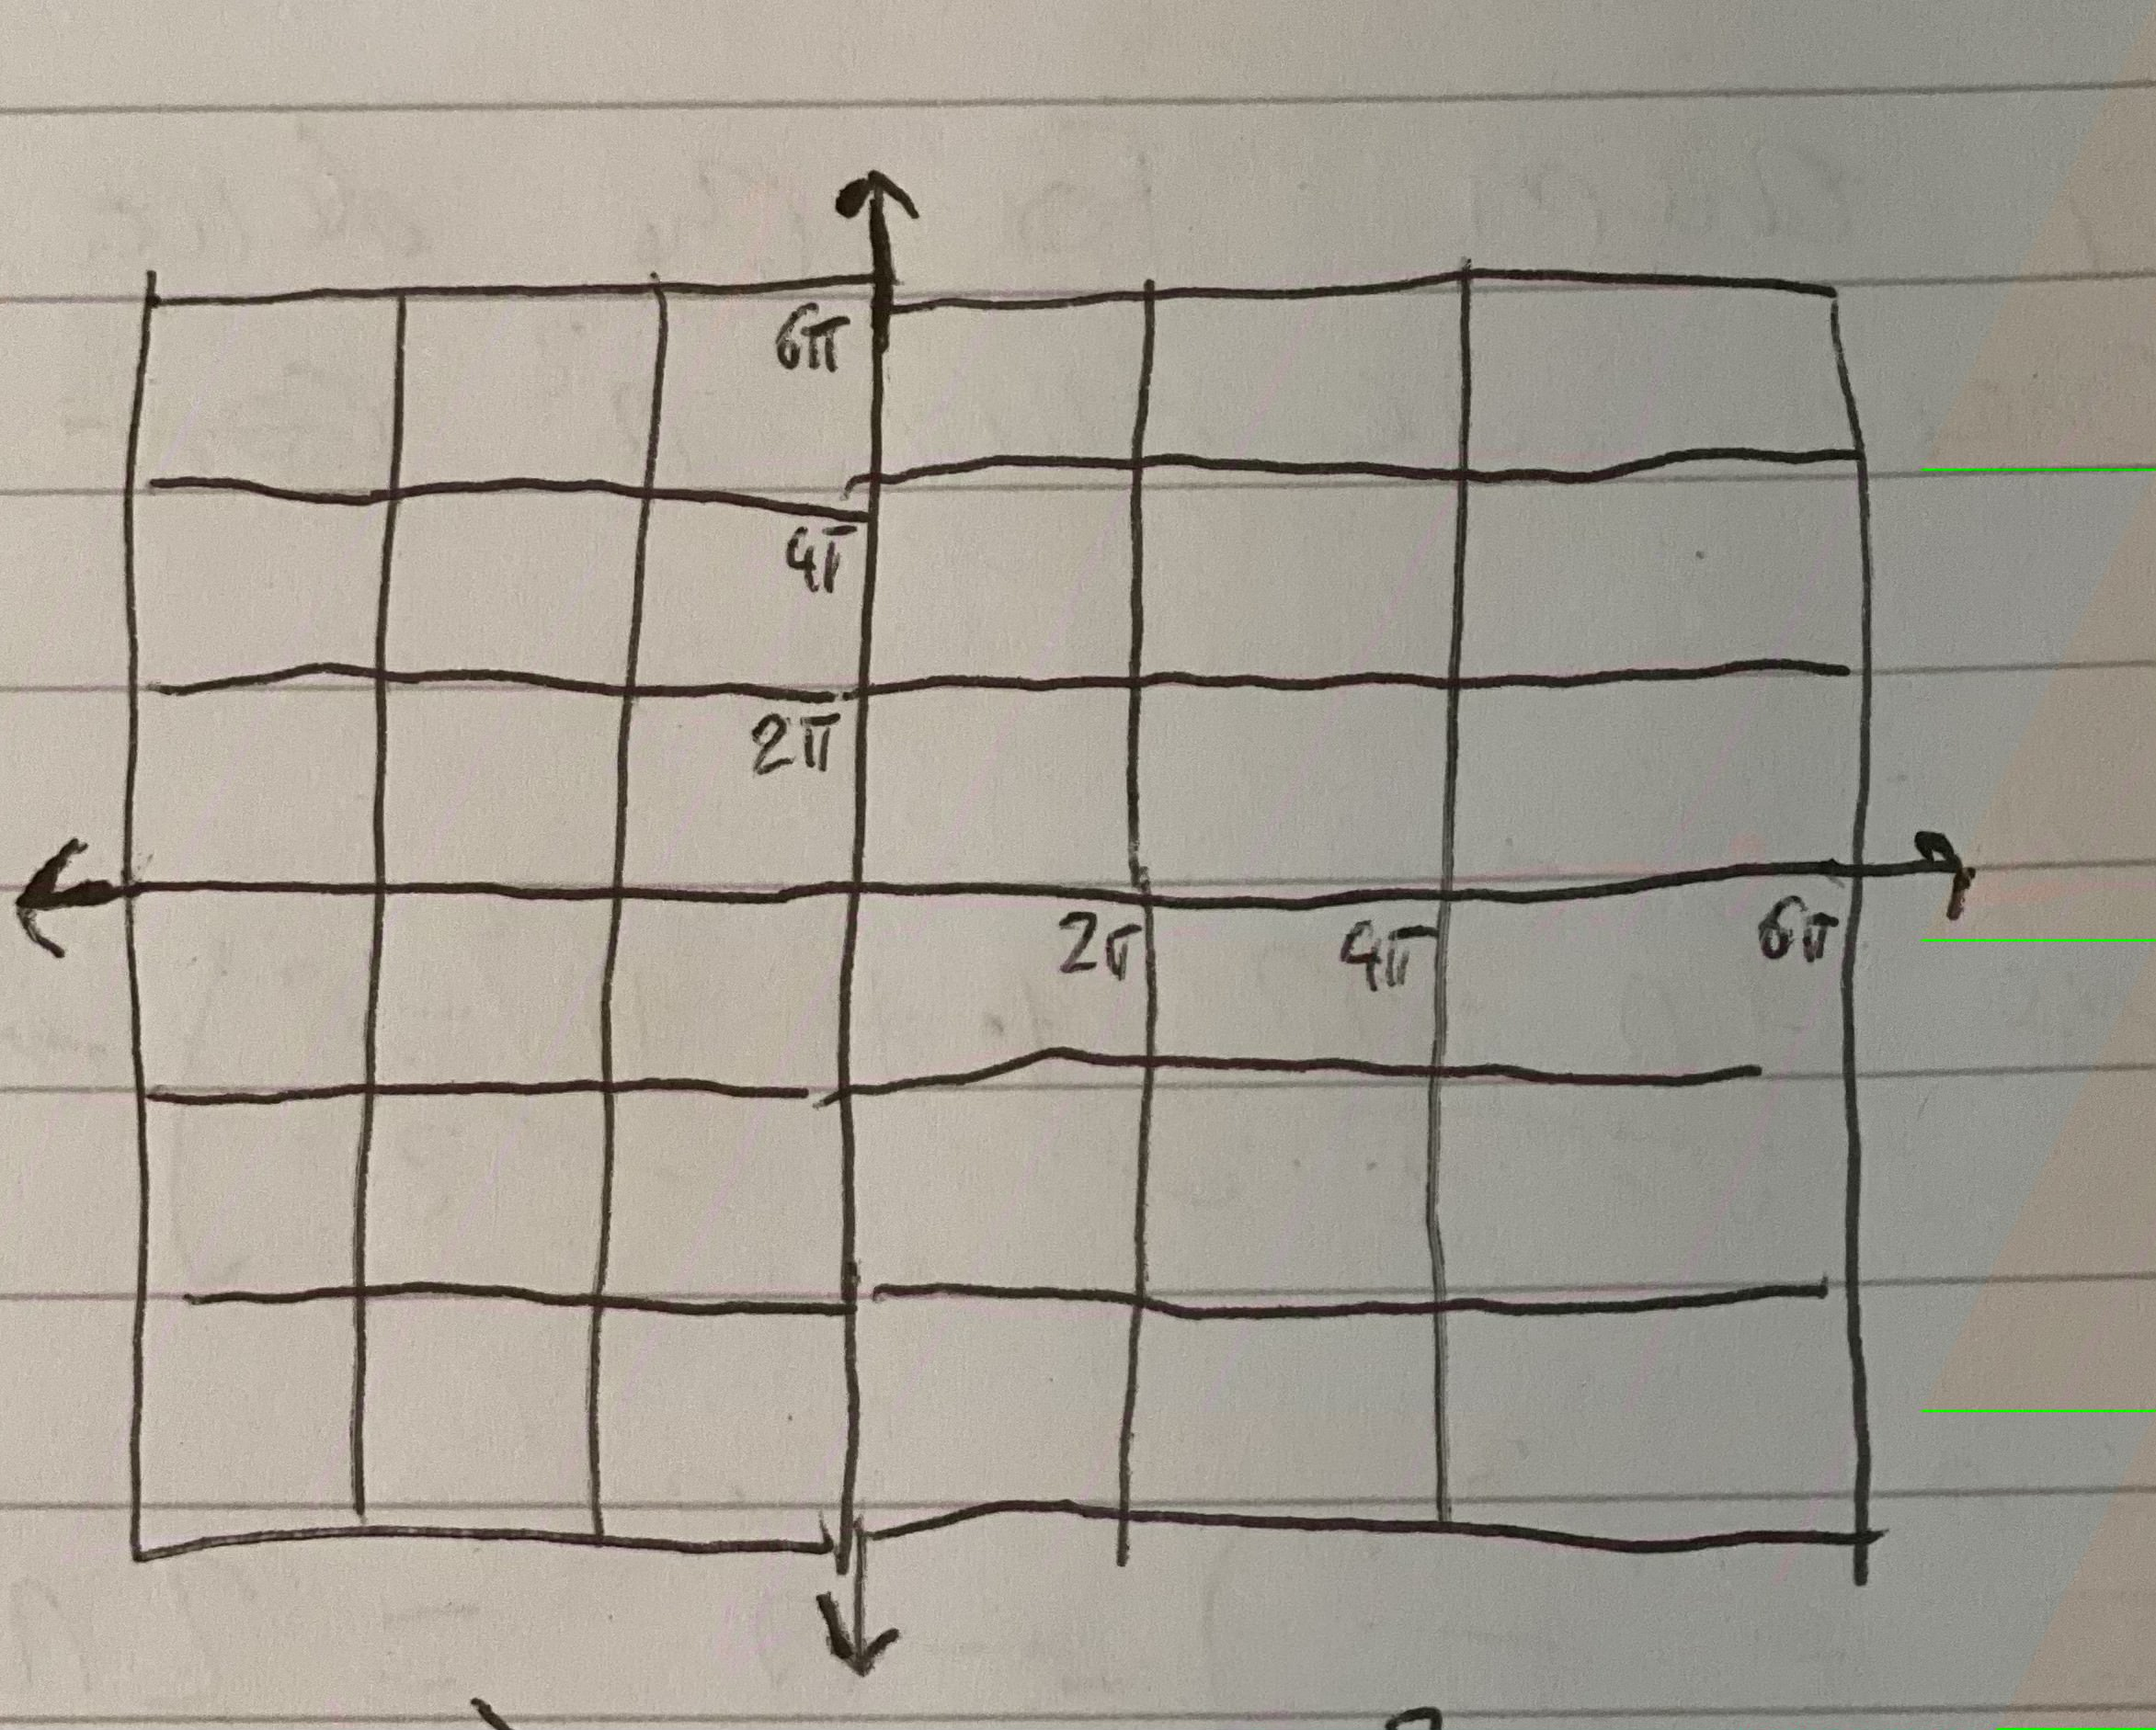
\includegraphics[width=8cm]{plot.jpg}
   \caption{Plot for question two showing how the action represents squares on an xy plane}
   \end{figure}

\item Question 3\\
To answer whether there is a subgroup $H$ of $U(5)$ we need to explore the different dimensions of A, as different dimensions of A will give different dimensions of H and thus different properties of $H$:
\\
\\
Consider the case where A has $dim A =0$, meaning that $x$ and $y$ are 0. This is a simple case as $H$ is all of $U(5)$ such that $H$ has dimensions $dim H = 5^2 = 25$. It is also a subgroup.
\\
\\
Consider the case where A only have 1 dimension, where $x \neq 0 $ and $y=0$ or $x=0$ and $y \neq 0$ or importantly showing linear dependence $y = cx \neq 0 \leftrightarrow x = cy \neq 0 $. A then has unit vector $v = \frac{x}{|x|}$ if x is 0, (if y is 0 then swap for ys) with an orthonormal basis in $\mathbb{C}^5$. In an orthonormal basis there exists a vector $u \in A$ such that
$$ u = \left( \begin{array}{ccccc} a & 0 & 0 & 0 & 0 \end{array} \right) $$
Of which $a \in \mathbb{C}$. A matrix $B \in H$ in which A is invariant and of course unitary $ B \in H \in U(5) $ can be represented by a block matrix with diagonal entries
$$  B = \left( \begin{array}{cc} e^{i\theta} & 0 \\ 0 & U_4 \end{array} \right) $$
Where $e^{i\theta} \in U(1) $ and $U_4 \in U(4) $ and thus $H$ is 
$$ H = \Big\{ B | e^{i\theta} \in U(1) \& U_4 \in U(4) \Big\} $$
$$ = \Big\{ \left( \begin{array}{cc} e^{i\theta} & 0 \\ 0 & U_4 \end{array} \right) | e^{i\theta} \in U(1) \& U_4 \in U(4) \Big\} $$
Which shows that $H$ is a proper subgroup with $dim H = dim U(1) + dim U(4) = 17 $
\\
Finally, the case where if both $x$ and $y$ don't equal 0 and are linearly independent. Again, if we have a orthonormal basis for A such that a vector $u \in A$ is
$$  u = \left( \begin{array}{ccccc} a & b & 0 & 0 & 0 \end{array} \right) $$
Then $B \in H$ has the block matrix form with diagonal entries:
$$ B = \left( \begin{array}{cc} U_2 & 0 \\ 0 & U_3 \end{array} \right) $$
So we have 
$$ H = \Big\{ \left( \begin{array}{cc} U_2 & 0 \\ 0 & U_3 \end{array} \right) | U_2 \in U(2) \& U_3 \in U(3) \Big\} $$
Which has dimension $dim H = dim U(2) + dim U(3) = 13 $ and is a proper subgroup. 
\item Question 4\\
\begin{enumerate}
   \item 

In $SL(2, \R)$ we have a matrix A such that 
$$ A = \left( \begin{array}{cc} x_0-x_1 & x_2+x_3  \\ x_2-x_3 & x_0+x_1  \end{array}\right) $$
Taking the determinant with the constraint $det(A) = 1$ 
$$ det(A) = (x_0 - x_1)(x_0 + x_1 ) - (x_2 + x_3 ) (x_2 - x_3) $$
$$ = x_0^2 - x_1^2 -x_2^2 + x_3^2 =1 $$
Now we have $-x_1^2$ and $-x_2^2$ which is not in the forn needed as they have negative constants in front of them. Multiplying by -1 to get into the form required gives us 
$$ -x_0^2 -x_3^2 + x_1^2 +x_2^2 = -1 $$ 
Giving $(c_0, c_n, c) = (-1,-1,-1)$ and $SL(2,\R)$ is a 3 dimensional anti-de sitter space $AdS_n$. 
\item Part b wasn't answered fully as I don't really understand Conjugacy Classes
\\
If $A \in SL(2,\R) $ we say that the conjugacy class of A is $A_{CL}$
$$ A_{CL} = \Big\{ B \in SL(2,\R)| S \in SL(2,\R): B= S^{-1} A S \Big\} $$
Where $S$ is a symmetric matrix and $B \in A_{CL} $
\\ B can be considered equivalent to A such that $A~B$ and in terms of traces $Tr(A) = Tr(B)$
\end{enumerate}
\item Given a group $G$, a left $G$-space $X$, and an element $x\in X$, prove that the isotropy group of $x$ is a subgroup of $G$.
\\
Let $G_x$ by the isotropy group of $G$. To be a subgroup we have that 
$$ \forall g_1 g_2 \in G \ g_1 g_2 \in G $$
$$ \forall g \in G \ g^{-1} \in G $$
Let $g_1 g_2 \in G_x $ such that the left action $L_{g_1} (x) = x \ L_{g_2} (x) = x $ where $L$ is a homomorphism
$$ L_{g_1g_2} (x) = L_{g_1} (L_{g_2}(x)) = L_{g_1} (x) = x$$
And this $g_1 g_2 \in G_x$. Note that this also proves associativity. For the second property of a subgroup lets state $g \in G_x$ such that
$$ L_{g^{-1}g}(x) = L_{g^{-1}} ( L_g (x)) = L_{g^{-1}} (x) $$
Thus $g^{-1} \in G_x$. 
\\
Hence $G_x$ is a subgroup of G. \\
Not entirely sure if this is true but if I say that the indentity element of $L$ such that $L_e = id_X$ then we can prove the existence of the identity element in $G_x$
$$ L_e(x) = id_X (x) = x $$
Hence $e \in G_x$ and $G_x$ is a group and thus a subset of $G$, solidying evidence that $G_x$ is a subgroup of $G$ 
\end{enumerate}


\end{document}
